\chapter{Background}
\label{chap:background}

In this chapter we are going to explain the most important concepts of the 
upcoming 5G standard, talking about the Virtual Network Functions (VNFs) and 
how first experiments with this new technology already begun. Finally we are 
going to briefly introduce and explain the technologies involved and their role.

\section{Network slicing}
A network slice can be defined as a logical virtual network, tailored for a
given use case, on the top a common network using technologies such as
Software-Defined Networking and Network Function Chaining that allows network
softwarization~\cite{ordonez2017network}. The notion of separated virtual
networks deployed on the same infrastructure is not new, e.g. VPN, but it has
some specifics that make it a novel idea. The concept of network slicing was
first introduced in 2002 in\cite{peterson2003blueprint}, where a network 
overlay that allows services to run continuously and to access the overlay
resources across different slices was illustrated.
Services operating over the overlay management have their own slice instead.
This idea was lately refined in 2016, where the design of network slicing was
based on a three-layers model~\cite{alliance2016description}, as depicted in 
Figure~\ref{chap:background:img:network_slicing}.

\begin{figure}
  \centering
  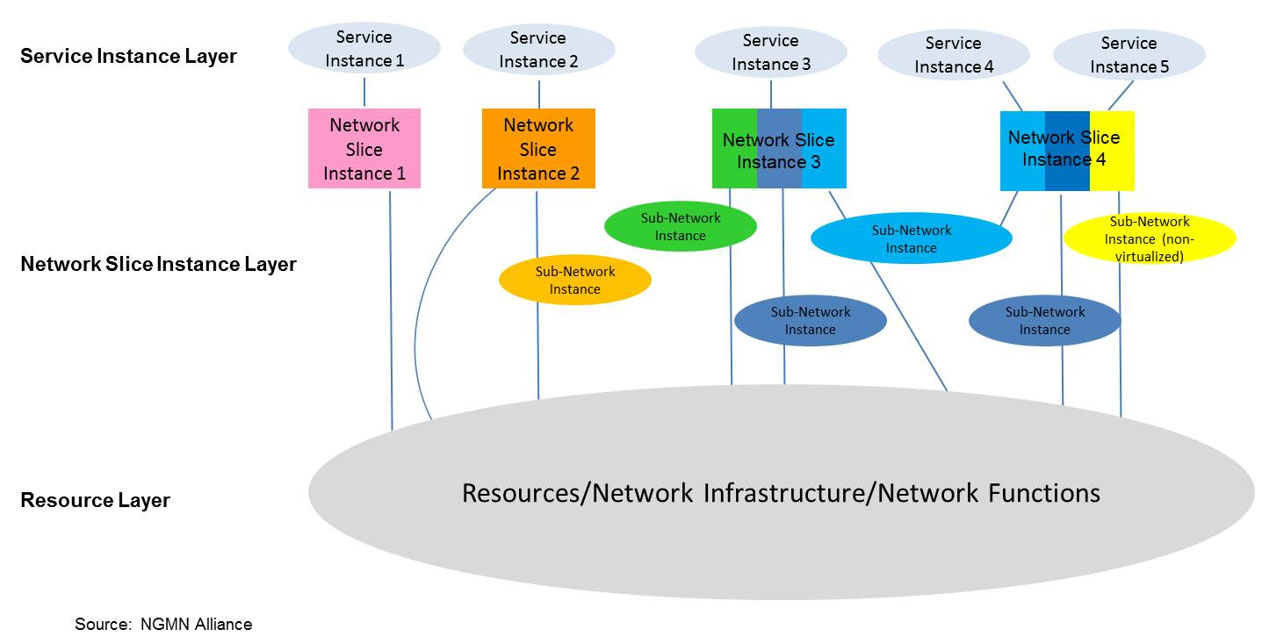
\includegraphics[scale=0.2]{networkslicing}
  \caption{The three layers model of network
  slicing~\cite{alliance2016description}}
  \label{chap:background:img:network_slicing}
\end{figure}

The first layer is the \emph{Service Instance Layer} used to represent the
business or user services supported, the second one is the \emph{Network Slice
Instance Layer}. This is a set of network functions that allows to
satisfy certain requirements~\cite{kotulski2017end}. Network functions, in
general, can be both physical, thus a combination of vendor-specific hardware
and/or virtualized. In that case the function is implemented as software and it
is decoupled from the hardware on which it is running on. Each instance must be
isolated, in order to ensure that function running at the top of it will always
provide the same Quality of Service, without degrading because of a change on
another slice~\cite{richart2016resource}. It also allows to provide better
security. In fact, in case of attack or fault of a certain slice, others must
not be affected. Moreover, each slice must implement it own set of security
function to preventing unauthorized access. Furthermore, isolation let to
manage individually each slice~\cite{ordonez2017network}. Network slice
instances are defined by a \emph{Network Slice Blueprint}: a complete
description of the structure and data flows that allow the creation and the
control of the Network Slice Instance during its whole lifecycle. The blueprint
also refers to the resources needed to assemble the network slice and defines
its characteristics (e.g. ultra-low latency, ultra-reliability, value-added
services for enterprises, etc.). The last layer is the \emph{Resource Layer},
containing both physical and logical resources, that involve all physical
assets and resources for computation, storage or transport, including radio
access.

\section{Software-defined networking}
The SDN is an emerging approach to cloud computing and networking technology
capable of supporting the dynamic nature of future network functions and
intelligent applications while lowering operating costs through simplified
hardware, software, and management~\cite{sezer2013we}, that allows to configure
network in a programmatically way, possibly enhancing monitoring and
performances. One of the main principles of SDN architecture is to decouple the
packet forwarding process, \emph{data plane}, from the routing one, the so
called \emph{control plane}. The architecture also contemplate that network
intelligence and state are logically centralized\cite{fundation2012software}. 

It has some drawbacks in terms of
security, scalability and elasticity, because of the centralized architecture.

\subsection{SDN stack}
\begin{figure}[ht]
 \centering
 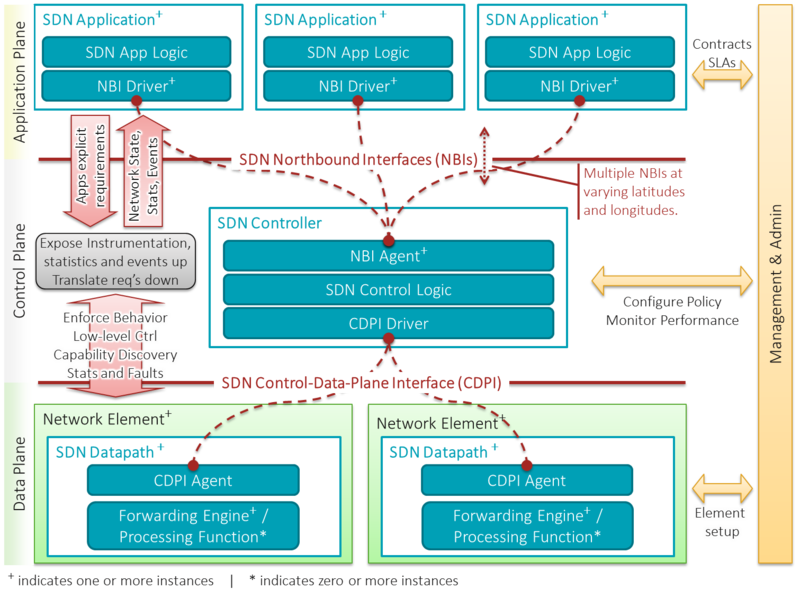
\includegraphics[scale=1.3]{sdn_architecture}
 \caption[SDN architecture schema]{SDN architecture schema. Is possible to 
denote the three layer logic: the Application plane, the Controller plane and 
the Data plane~\cite{fundation2013software}.}
 \label{chap:background:img:sdn_architecture}
\end{figure}
As depicted in Figure~\ref{chap:background:img:sdn_architecture} the SDN
architecture can be split in three different layers, also known as planes,
based on their functionalities~\cite{fundation2012software} as explained
in~\cite{fundation2013software}.

\subsubsection{Application plane}

In the \emph{Application plane} lays \emph{SDN applications} that are programs
whose role is to set the behavior of the SDN controllers 
and manage its hardware resources and data through APIs, often called 
\emph{northbound interfaces} (NBI). In order to do so they can also build an
abstracted view of the network, using controllers information, in order to make
the traffic analysis easier and to simplify the decision making process..
These interfaces provide an additional abstraction layer that high-level 
applications can consume, enabling the possibility to use a variety of 
different vendors' controllers in the same way. Applications consists both of
the two defined layers, one that is responsible to manage the whole logic, and
another one dedicated to the communication part, that in particular uses the
previously defined NBIs.

\subsubsection{Controller plane}

\emph{SDN controllers}, are logically centralized components that
receive requests from SDN applications and either translate them 
in a fashion that can be understood from the SDN Datapath, or collect 
data as statics and events needed by the application to build an abstract view
of the network. 
Due to the variety of tasks a controller has to accomplish, its logical 
subdivision is achieved with a three-layer architecture, in which every layer 
exposes it's own interface, that can be consequently used by the upper 
layers, up to the \emph{NBI agents}.
NBI agent manages the communications with SDN applications, exposing interfaces
to access network data and to the set of the controller functionalities.
In particular, the middle layer represents the \emph{SDN Controller Logic},
which process the requests coming from the upper layer applications. Finally
requests are communicated to the remaining network components, exploiting the
Control to Data-Plane Interface driver.

Despite the centralized design of controllers there are no limitations on the
implementation, so it possible to create federations of controllers or organize
them into a hierarchy.

\subsubsection{Data plane}
In the lowest plane we can find the \emph{SDN Datapath}, defined as a logical
network device, which exposes the possibility to access and control to its
forwarding and processing capabilities.It is composed by a CDPI agent and a set
of one or  multiple traffic forwarding engines and of a zero or more traffic
processing functions, that are, as a matter of fact, the devices logic.
Datapath can be mapped either to a single physical device or multiple ones and
the implementation of the its logic does not preclude neither the
virtualization or the sharing of physical resources nor the interoperability
with non-SDN networking.

\subsection{OpenFlow protocol}
The SDN strategy is often associated with the OpenFlow protocol because it is
the first standard communications interface defined between the control and the
datapath in SDN architecture~\cite{fundation2013software}, making possible to
access from controller the components of infrastructure, such as switches and
routers. OpenFlow enables the remote administration of networks working on 
layer 3: packets forwarding tables can be modified relying on packet matching 
rules. Following this approach it is possible to change routes periodically or 
ad-hoc, based on packet types, traffic or network load.

\begin{figure}[t]
 \centering
 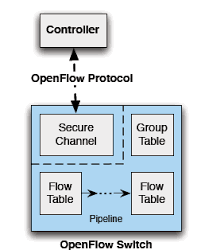
\includegraphics[scale=0.65]{openflow}
 \caption{OpenFlow protocol communication graph}
 \label{chap:background:img:openflow_protocol}
\end{figure}

In Figure~\ref{chap:background:img:openflow_protocol} it is possible to see the
how switches works in the OpenFlow protocol. Basically, OpenFlow switches own a
set of tables to organized packet control and forwarding. These tables can be
updated by higher-level application, usually an SDN application or controller,
taking advantage of OpenFlow channels (called OF channels). 

\section{Virtualization}
Cloud computing is nowadays one of the cutting edge Internet technologies, and
it is possible thanks to virtualization, that allows to isolate applications,
optimizing the utilization of hardware resources and providing more flexibility.
Virtualization, in computing, usually refers to the act of creating a virtual
version of a certain asset, such as virtual computer hardware platform,
operating system (OS), storage device, or computer network
resources~\cite{liu2014research}. Conventional virtualization
(hypervisor-based) uses virtual machines: it provides strong isolation and a
complete operating system~\cite{eder2016hypervisor}. In hypervisor
virtualization every pieces of hardware required to running software is
emulated, and it is common that the hypervisor provides interfaces to access
the real hardware, for instance to access physical devices or to communicate
with the network. However all this functionalities comes to a resource
overhead~\cite{scheepers2014virtualization}Container-based virtualization,
instead, could be a more efficient in certain context, because it does not
emulate the entire computer. A container is seen as an isolate process running
on the host, to which the Linux kernel gives a set of capabilities.

\subsection{Network Virtualization}
Virtualization, in the networking context, refers to the act of combining
hardware, software and functionalities into a virtual network. This abstraction
runs on the top of a physical network in a hyper-visor, decoupling the logical
network from the hardware one. Network virtualization allow multiple,
heterogeneous networks to cohabit, increasing the flexibility and manageability.
The idea of network virtualization came from the decoupling of the role of the
traditional ISP into two different entities: who provides the infrastructure
(InPs) and who provides the services(SPs). In that context it is possible to
aggregate resources, even from different InPs, creating a virtual network,
offering an end-to-end service~\cite{chowdhury2009network}. Most known
instances of NV are \emph{VPNs}, dedicated networks that allows the
communication among multiple sites, using
private and secure tunnels, relying on the public network such as Internet.
Other examples of network virtualization are \emph{overlay networks}. They are
logical networks, build on the top of an existing physical network, typically
implemented at the application layer. 


\subsection{Network Function Virtualization}
The \emph{Network Function Virtualization} (NFV) concept refers to the use of 
virtualization technologies to virtualize network nodes functions. This
emerging technology focuses on the decoupling of function logic and hardware,
allowing VNFs to run on the top of servers, switches, storage 
devices or on cloud computing infrastructures. In other word the software logic
is separated from the custom platform on which it runs, enabling the use of
commodity hardware~\cite{gray2016network}.
That approach worked well in the past, because of the need to follow rigorous 
standards, providing at the same time high quality, but it led to long product 
cycles and high specialized services that use a combination of software and
hardware resources, typically vendor-specific, and only largely
non-interoperable within other vendor solutions. New Internet scenarios, that 
include IoT and the increasing number of services to spread multimedia data 
(Skype, Netflix, Spotify, \dots), requires more flexible functions and faster 
network deployments. 
This detachment provides greater flexibility to scale VNF based on traffic and
performances and also improve the automation of function deploy and update:
removing dedicated hardware also will reduce costs machines and for
maintenance. 


The NFV technology is exploited in a framework, organized
at least by three components~\cite{etsi2013gs}, as represented in
Figure~\ref{chap:background:img:etsi_arch}:
\begin{enumerate}
  \item a software, able to run on over the NFVI, that performs the network
  function that must be deployed, that is the VNF;
  \item NFV Infrastructure (NFVI) that is composed by all physical resources
  and how these can be virtualized, that forms the environment where the VNFs
  are deployed;
  \item NFV Management And Orchestration (NFV-MANO) that covers the
  orchestration and management of both physical and logical resources, the
  functional blocks, data repositories used by these blocks, reference points
  and interfaces through which these functional blocks exchange
  information for the purpose of managing and orchestrating NFVI and VNFs.
\end{enumerate}

\begin{figure}
  \centering
  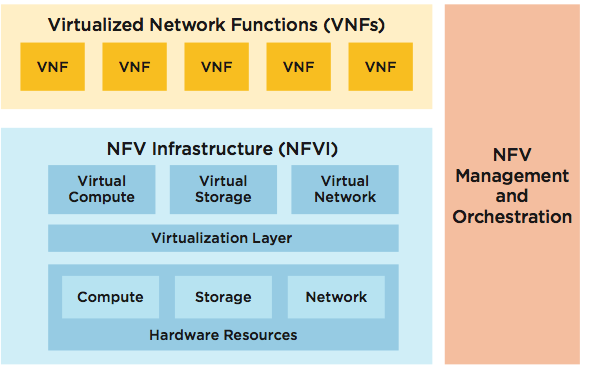
\includegraphics[scale=2]{etsi_arch}
  \caption{Network Function Virtualization reference
  architecture~\cite{etsi2013gs}}
  \label{chap:background:img:etsi_arch}
\end{figure}

\subsection{Network Function Virtualized Infrastructure}
As mentioned before, NFVI is the combination of physical and logical resources,
that combined together create the environment on which the VNFs are deployed
and run. Physical supplies can be proprietary systems, commercial-off-the-shelf
hardware, software and network resources or cloud computing capabilities. The
abstraction of resources is made taking advantage of a virtualization layer,
that hides the underlying infrastructure. Storage and computing resources may
be represented in terms of virtual machines or
containers~\cite{mijumbi2016network}.


\subsection{VNF challenges}
This new concept open a plethora of challenges~\cite{han2015network}. Regarding
performances, functions running on general purposes servers cloud affect
throughput and latency, moreover the capacity of the virtualized function can
be less than the hardware and software version. To reach comparable levels in
terms of performances efficient algorithms are needed, as a excellent resource
management. Another problems is the VNF management. In case of hardware
functions resources are almost equivalent, at the contrary, virtualized ones
could have costs and values that differs significantly depending on the point
of presence on which are deployed. On the other hand, since VNFs are software
components, can elastically scale up and down, depending on the traffic loads
and user demand. Another management challenge refers to keeping track where the
VNF is running, that is of paramount importance in case of issues. Related to
possible dysfunctions, software function must reach a certain level of
reliability. Generally, purpose-build network equipment can ensure the
five-nines reliability requirement, that is more challenging to follow in that
scenario due to the higher number of possible points of failure, such as during
the scaling operation or VNF migrating from a point of presence to another.
Finally even security must be taken into account. In fact, infrastructure on
which VNFs run can be outsourced to third parties. Furthermore, orchestration
and management components must implement some sort of intrusion prevention and
detection system and the sharing of resources can introduce security threads.

\section{The upcoming connectivity standard: 5G}
The continuous innovation in the mobile network connectivity is leading to the
creation of a new standard, the 5G, which is estimated to arrive to the market
consumer in 2020\todo{CITE}. Lead by the Next Generation Mobile Network (NGMN)
alliance, a group composed by the major players in the field of mobile
connectivity, the 5G aims to offer not only at the end-user a new way to browse 
the web, download and watch interactive content but also to create an ad-hoc 
solution for Machine-to-Machine (M2M) data traffic, which is increasing more 
than ever thanks to the spreading of IoT devices, which sensors need to 
continuously send data to servers/data-centers. Relatively to LTE\todo{Explain 
acronym}, 5G points to have data rates $10$ times better, with $10$ times 
smaller end-to-end latency and an increased connection density by $100$ 
times\todo{CITE}.

\begin{table}[t]
\centering
\resizebox{\textwidth}{!}{%
  \begin{tabular}{p{4,5cm}|p{5,5cm}|p{5cm}}
\textbf{Attribute}                                                    & 
\textbf{LTE capability}                                                         
 
                                                                           & 
\textbf{Improvement needed to meet NGMN requirements}                 \\ \hline
\textbf{Data rate (per user)}                                         & Up to 
100 Mb/s on average Peaks of 600 Mb/s (Cat 11/12).                              
 
                                                                     & 10X 
expected on average and peak rates and 100X expected on cell edge \\
\textbf{End-to-end latency}                                           & 10 ms 
for two-way RAN (pre-scheduled). Typically, up to 50 ms end-to-end if other 
factors are considered (e.g., transmission, CN, internet, proxy servers). & 10X 
(smaller)                                                         \\
\textbf{Mobility}                                                     & 
Functional up to 350 km/h (for certain bands up to 500 km/h). No support for 
civil aviation.                                                                
& 
1.5X                                                                  \\
\textbf{\begin{tabular}[c]{@{}l@{}}Connection\\ density\end{tabular}} & 
Typically $\sim$2,000 active users/km2.                                         
 
                                                                           & 
100X                                                                 
\end{tabular}%
}
\caption[5G improvement over LTE]{An extract from the official 5G white paper 
illustrating the improvements of 5G relatively to LTE connections.}
\label{chap:intro:table:ltevs5g}
\end{table}

Part of the new requirements can be satisfied using a large radio spectrum with
higher frequencies. The utilization of higher frequencies, though, mean that the
radio signals can be easily disrupted by physical objects, like buildings and
many geographical elements (such as hills and mountains), clashing with the
expectation of an ever-reachable connectivity. It is here where virtualization
plays an important role. In fact, the re-design of some network components today
existing via hardware can transform a monolithic networking approach to a 
modular one, exploiting the flexibility that Virtual Network Functions 
(VNFs)\todo{CITE VNF-P: A Model for Efficient Placement of Virtualized Network 
Functions} can offer thanks to virtualization, closing the gap to the use-case 
fulfillment defined by the NGMN alliance\todo{CITE: NGMN View on 5G 
architecture} which require a decreased time to set up and deploy network 
services (specifically, from 90 hours to 90 minutes\todo{Search this 
requirement, check 90h 'cause I'm not sure about it}).

\subsection{5G architecture}

With the constraints placed on the requirements formulated by the NGMN alliance,
5G envisage a multi-layered architecture, based on three main layers:\todo{CITE:
  NGMN View on 5G architecture}
\begin{itemize}
\item \textbf{infrastructure resource layer}: physical resources that are 
exposed via a virtualized interface, and that can be monitored using specific 
APIs
\item \textbf{business enablement layer}: where a library of functions and
  deployment is contained, and its configuration is accessible via APIs
\item \textbf{business application layer}: layer that contains specific
  applications and services of the operator
\end{itemize}

\todo{Add three-layer image here?}

This separation in layers allows to easily manage multiple identities 
differently: an Internet Service Provider (ISP) could manage a multitude of 
physical infrastructures and have multiple business enablements dislocated 
along an entire continent for example, but it could decide to have only a 
single centralized business application deployment that manage all the other 
layers resources.

\subsubsection{Network slicing}
The role of a ``network slice'' in a 5G architecture is to specifically handle 
the Control-plane\todo{Explain what a control plane is?} of a particular 
service (e.g. smartphones traffic, autonomous driving, massive IoT), deploying 
resources in a manner that assure the required latency, security and 
reliability. While some very peculiar legacy services could require specific 
hardware, the common resources between services could be shared in a 
virtualized way, providing auto-scaling capabilities in services that are under 
heavy network pressure.

\section{The VIBES project}
 
 This thesis is part of the VIBES project\todo{Talk about VIBES project, add
   some reference, explain what it is.}, where the necessity for better TCP/IP
 transmission through satellite connections is the main requirement. To reach
 this goal, the project specifications suggest to exploit the 5G incoming
 technology and use the NFV-MANO architecture to perform first packets
 elaboration and performance improvement and finally TCP/IP satellite chunk
 optimization with the Performance Enhancing Proxy (PEP). The VIBES project
 proposed five technical requirements:
\begin{enumerate}
 \item Analysis of the applicability of current and new Internet protocols in
   the proposed VNF-PEP architecture
 \item Implementation of a VNF-PEP prototype
 \item Building of a PoC test platform
 \item VNF-PEP validation and performance tests on 5G use-cases
 \item Demonstration test-bed management
\end{enumerate}

\begin{figure}[t]
 \centering
 
\includegraphics[scale=1]{vibes_logo}
 \caption{ViBeS project logo}
 \label{chap:background:img:vibes_logo}
\end{figure}


\subsection{VNF-PEP architecture and internet protocols}

The analysis of this topic revealed to be trivial: since internet has many
different protocols that would become infeasible to support all of them at the
same time, packet encapsulation present itself as the only feasible solution:
every packet incoming in the VNFs has already been encapsulated by a generic
packet encapsulator/decapsulator,
\todo{Also I think that the main purpose of UDP encapsulation is not to hide 
the protocol used on the edges but 1) use a ``quick protocol to exchange data 
among VNFs and 2) we are hiding the path not the protocol itself. As we were 
discussing, we are creating some sort of proxy, so the aim will be the same 
even if we support a plethora of protocols.''} making the whole architecture 
independent from the protocol a particular flux of data. To achieve this, 
several solutions have been studied, and at the end packet encapsulation with 
TCP split (for TCP sessions) have been chosen. The rationale that guided us on 
this choice is described in Chapter~\ref{chap:vnf_ns_impl}. \todo{Update 
reference with the section of the explanation}

\subsection{VNF-PEP prototype}

Since the requirement for the whole system (MANO+PEP) were too challenging, the 
goal shifted into creating a MANO test-bed and a working NFVI, excluding PEP. 
The VNF architecture was shaped following the container orchestrator we decided 
to use. An more detailed architectural implementation can be found at 
Chapter~\ref{chap:archimpl}.

% \section{Technologies used}

\vspace{0.5cm}

Starting with the first step of creating a MANO able to process incoming data
packets through VNF functions, we encountered that many networking tools already
present in the market required some tweaking and some integration, shifting our
goal to create a complete European Telecommunications Standards Institutes
(ETSI) Management and orchestrator (MANO) test-bed instead, following the
specifications suggested in the RFC 7665, thus implementing only the first three
requisites, without digging in the satellite data flow optimization. In
particular, we discovered how, these tools, were suitable to create ETSI MANO
and VNFs using virtual machine or exploiting cloud technologies, while they were
not designed with enough flexibility an integration with Docker. In the next
chapter we are going to take a deep analysis of the cited technologies 
(Section~\ref{chap:prjan:sec:tech}, in order to provide to the reader enough 
context to be able to understand our design choices we are going to describe 
later.

\noindent With this in mind, we performed a requirements analysis described in
the next chapter.\todo{This should be put at the end of the introduction.}
 
